%/////////////////////////////////////////////////
%/
\chapter{Experimental Results}
%/
%/////////////////////////////////////////////////
\label{chap:experimental_result}

%/////////////////////////////////////////////////
%/
\section{Experimental Setup}
%/
%/////////////////////////////////////////////////
We evaluate our implementation by running some benchmarks over different strategies as well as solvers.
We have used QF\_NRA benchmarks \cite{SMTLIB-benchmarks} from SMT-LIB \cite{BarFT-SMTLIB}.
We run the benchmarks on a cluster having multiple processors of 2.10 GHz Intel Xeon Platinum 8160 and 8GB of memory per process.
We decided to use a timeout of 120 seconds (s) per problem instance for the experiment.

%/////////////////////////////////////////////////
%/
\section{Results}
%/
%/////////////////////////////////////////////////
We have already described in the section \ref{subsubsec:Module_Settings} that we use different strategies \textit{NRARefinementSolver$1$}, \textit{NRARefinementSolver$2$}, $\dots$, \textit{NRARefinementSolver$21$} which are mentioned as  smtrat$1$, smtrat$2$, $\dots$, smtrat$21$, respectively in this chapter. 
The results for smtrat$1$, smtrat$2$, $\dots$, smtrat$21$ without preprocessing (WoP) are reported in Table \ref{table:results_our_solvers} where the first column contains the solver's name.
The second and third column contain the number of satisfiable and unsatisfiable instances that could solve within the time limit, respectively with average solving time.
The total number of solved instances with the percentage of the solution is reported in the last column from worst to best.
The detailed settings of each solver are also provided in Table \ref{table:ourSolvers_heuristics_sequences} by a pair of heuristic type and sequence of axiom types (Section \ref{subsubsec:Module_Settings}).\newline

\noindent Table \ref{table:results_our_solvers} shows some interesting aspects.
The solver smtrat4 performs the best, whereas smtrat7 performs the worst.
However, smtrat11 and smtrat3 solve the highest number of satisfiable and unsatisfiable instances, respectively.
It is noticeable that six solvers of heuristic type \textit{ALL} which is marked green perform the best in a row.
On the other hand, the red marked rows highlight all solvers of heuristic type \textit{RANDOM} perform worse than other solvers in a row.
Also, this group of solvers solves less unsatisfiable instances compared to other solvers.
We can see that smtrat7, smtrat14 and smtrat21 share same sequence of axiom types from Table \ref{table:ourSolvers_heuristics_sequences}.
Interestingly, two solvers smtrat7 and smtrat21 among these three solvers rank at the last which demonstrates that sequence $7$ is not effective because it has the most  expensive axiom monotonicity at the very beginning of the sequence.
Sequence $4$ is followed by both our best solver smtrat4 and the highest number of satisfiable instances solving solver smtrat11.
Moreover, smtrat4 and smtrat11 take less solving time on average for both instances than most of the solvers.
So, it can be said that sequence $4$ is the most effective sequence where our defined axiom ICP is placed at the beginning and ICP helps to reach the solution more quickly.
It also can be said that a pair of heuristic type ALL and sequence $4$ helps to improves the performance of a solver.
Therefore, we decide to consider smtrat4  for further evaluation which follows heuristic type ALL to collect unsatisfiable axioms by performing refinement over sequence $4$.\newline

\begin{table}[]
    \caption{Number of solved instances for our solvers without preprocessing (WoP)}
    \centering
    \begin{tabularx}{\textwidth}{lXrrXrrXrr}
    	\toprule
    	\textbf{Solver}
    	&& \multicolumn{2}{c}{\textbf{SAT}}
    	&& \multicolumn{2}{c}{\textbf{UNSAT}}
    	&& \multicolumn{2}{c}{\textbf{Overall}}
    	\\
    	\midrule
    	\rowcolor{black!20}
    	smtrat7
    	&& 1678 & 2.53~s
    	&& 3806 & 1.88~s
    	&& 5484 & 47.7~\%
    	\\ 
    	\rowcolor{black!20}
    	smtrat21
    	&& 1735 & 3.06~s
    	&& 3759 & 1.91~s
    	&& 5494 & 47.8~\%
    	\\
    	\rowcolor{red!20}
    	smtrat13
    	&& 1867 & 1.12~s
    	&& 3659 & 1.12~s
    	&& 5526 & 48.1~\%
    	\\
    	\rowcolor{red!20}
    	smtrat14
    	&& 1893 & 1.68~s
    	&& 3646 & 1.19~s
    	&& 5539 & 48.2~\%
    	\\
    	\rowcolor{red!20}
    	smtrat9
    	&& 1899 & 1.39~s
    	&& 3659 & 1.30~s
    	&& 5558 & 48.4~\%
    	\\
    	\rowcolor{red!20}
    	smtrat10
    	&& 1895 & 1.54~s
    	&& 3664 & 1.30~s
    	&& 5559 & 48.4~\%
    	\\
    	\rowcolor{red!20}
    	smtrat12
    	&& 1902 & 1.61~s
    	&& 3657 & 1.14~s
    	&& 5559 & 48.4~\%
    	\\
    	\rowcolor{red!20}
    	smtrat11
    	&& 1916 & 1.21~s
    	&& 3663 & 1.17~s
    	&& 5579 & 48.6~\%
    	\\
    	\rowcolor{red!20}
    	smtrat8
    	&& 1914 & 1.39~s
    	&& 3669 & 1.24~s
    	&& 5583 & 48.6~\%
    	\\
    	\rowcolor{blue!20}
    	smtrat16
    	&& 1801 & 1.94~s
    	&& 3818 & 1.84~s
    	&& 5619 & 48.9~\%
    	\\
    	\rowcolor{blue!20}
    	smtrat20
    	&& 1813 & 1.70~s
    	&& 3810 & 1.83~s
    	&& 5623 & 48.9~\%
    	\\
    	\rowcolor{blue!20}
    	smtrat17
    	&& 1809 & 1.99~s
    	&& 3827 & 1.92~s
    	&& 5636 & 49.1~\%
    	\\
    	\rowcolor{blue!20}
    	smtrat19
    	&& 1831 & 1.83~s
    	&& 3816 & 1.83~s
    	&& 5647 & 49.2~\%
    	\\
    	\rowcolor{blue!20}
    	smtrat18
    	&& 1817 & 2.28~s
    	&& 3840 & 2.10~s
    	&& 5657 & 49.2~\%
    	\\
    	\rowcolor{blue!20}
    	smtrat15
    	&& 1859 & 2.34~s
    	&& 3826 & 2.04~s
    	&& 5685 & 49.5~\%
    	\\
    	\rowcolor{green!20}
    	smtrat6
    	&& 1811 & 1.84~s
    	&& 3911 & 1.99~s
    	&& 5722 & 49.8~\%
    	\\
    	\rowcolor{green!20}
    	smtrat5
    	&& 1828 & 1.94~s
    	&& 3897 & 1.76~s
    	&& 5725 & 49.8~\%
    	\\
    	\rowcolor{green!20}
    	smtrat1
    	&& 1820 & 1.79~s
    	&& 3908 & 1.61~s
    	&& 5728 & 49.9~\%
    	\\
     	\rowcolor{green!20}
    	smtrat2
    	&& 1827 & 1.99~s
    	&& 3902 & 1.75~s
    	&& 5729 & 49.9~\%
    	\\
    	\rowcolor{green!20}
    	smtrat3
    	&& 1810 & 1.73~s
    	&& 3924 & 2.17~s
    	&& 5734 & 49.9~\%
    	\\
     	\rowcolor{green!20}
    	smtrat4
    	&& 1849 & 1.64~s
    	&& 3914 & 1.67~s
    	&& 5763 & 50.2~\%
    	\\
    	\bottomrule
    \end{tabularx}
    \label{table:results_our_solvers}
\end{table}

\begin{table}[]
    \centering
    \caption{Settings of our solvers}
    \begin{tabular}{|c|c|c|}
    \hline
    \textbf{Solver}                & \textbf{Heuristic type}                           & \textbf{Sequence no / Sequence of axiom types}                                                       \\ \hline
    smtrat1                        & \multirow{7}{*}{ALL}                         & 1 / zero, tangent plane, ICP, congruence, monotonicity                      \\ \cline{1-1} \cline{3-3} 
    smtrat2                        &                                              & 2 / tangent plane, zero, ICP, congruence, monotonicity                      \\ \cline{1-1} \cline{3-3} 
    smtrat3                        &                                              & 3 / tangent plane, ICP, zero, congruence, monotonicity                      \\ \cline{1-1} \cline{3-3} 
    smtrat4                        &                                              & 4 / ICP, zero, tangent plane, congruence, monotonicity                      \\ \cline{1-1} \cline{3-3} 
    smtrat5                        &                                              & 5 / ICP, tangent plane, zero, congruence, monotonicity                      \\ \cline{1-1} \cline{3-3} 
    smtrat6                        &                                              & 6 / congruence, zero, tangent plane, ICP, monotonicity                      \\ \cline{1-1} \cline{3-3} 
    smtrat7                        &                                              & 7 / monotonicity, zero, tangent plane, ICP, congruence                      \\ \hline
    \multicolumn{1}{|l|}{smtrat8}  & \multicolumn{1}{c|}{\multirow{7}{*}{RANDOM}} & \multicolumn{1}{l|}{1 / zero, tangent plane, ICP, congruence, monotonicity} \\ \cline{1-1} \cline{3-3} 
    \multicolumn{1}{|l|}{smtrat9}  & \multicolumn{1}{l|}{}                        & \multicolumn{1}{l|}{ 2 / tangent plane, zero, ICP, congruence, monotonicity} \\ \cline{1-1} \cline{3-3} 
    \multicolumn{1}{|l|}{smtrat10} & \multicolumn{1}{l|}{}                        & \multicolumn{1}{l|}{3 / tangent plane, ICP, zero, congruence, monotonicity} \\ \cline{1-1} \cline{3-3} 
    \multicolumn{1}{|l|}{smtrat11} & \multicolumn{1}{l|}{}                        & \multicolumn{1}{l|}{4 / ICP, zero, tangent plane, congruence, monotonicity} \\ \cline{1-1} \cline{3-3} 
    \multicolumn{1}{|l|}{smtrat12} & \multicolumn{1}{l|}{}                        & \multicolumn{1}{l|}{5 / ICP, tangent plane, zero, congruence, monotonicity} \\ \cline{1-1} \cline{3-3} 
    \multicolumn{1}{|l|}{smtrat13} & \multicolumn{1}{l|}{}                        & \multicolumn{1}{l|}{6 / congruence, zero, tangent plane, ICP, monotonicity} \\ \cline{1-1} \cline{3-3} 
    \multicolumn{1}{|l|}{smtrat14} & \multicolumn{1}{l|}{}                        & \multicolumn{1}{l|}{7 / monotonicity, zero, tangent plane, ICP, congruence} \\ \hline
    smtrat15                       & \multirow{7}{*}{FIRST}                       & 1 / zero, tangent plane, ICP, congruence, monotonicity                      \\ \cline{1-1} \cline{3-3} 
    \multicolumn{1}{|l|}{smtrat16} &                                              & \multicolumn{1}{l|}{ 2 / tangent plane, zero, ICP, congruence, monotonicity} \\ \cline{1-1} \cline{3-3} 
    smtrat17                       &                                              & 3 / tangent plane, ICP, zero, congruence, monotonicity                      \\ \cline{1-1} \cline{3-3} 
    smtrat18                       &                                              & 4 / ICP, zero, tangent plane, congruence, monotonicity                      \\ \cline{1-1} \cline{3-3} 
    smtrat19                       &                                              & 5 / ICP, tangent plane, zero, congruence, monotonicity                      \\ \cline{1-1} \cline{3-3} 
    smtrat20                       &                                              & 6 / congruence, zero, tangent plane, ICP, monotonicity                      \\ \cline{1-1} \cline{3-3} 
    \multicolumn{1}{|l|}{smtrat21} &                                              & \multicolumn{1}{l|}{7 / monotonicity, zero, tangent plane, ICP, congruence} \\ \hline
    \end{tabular}
    \label{table:ourSolvers_heuristics_sequences}
\end{table}

\noindent Table \ref{table:smtrat4_vs_mathsatAndZ3} has the same structure as Table \ref{table:results_our_solvers}.
Here we compare smtrat4 with other two SMT solvers z3 \cite{10.1007/978-3-540-78800-3_24} and mathsat \cite{ 10.1007/978-3-642-36742-7_7}.
We have taken two versions of smtrat4 which are without preprocessing (WoP) and with preprocessing (WP).
In order to compare the heuristics without external influence of other modules, we switched off preprocessing.
Smtrat4 WoP and WP both get the same original inputs but switching on preprocessing help.
So, for compatibilty we add also a version WP.
It is clearly visible that z3 and mathsat have excellent performance than smtrat4 in all cases.
The SMT solver z3 implements expensive and complete techniques based on variants of cylindrical algebraic decomposition \cite{Cimatti:2018:ILS:3274693.3230639}.
The SMT solver mathsat implements the incremental approach as described in \cite{irfan2018incremental} which was a PhD thesis and we have implemented the same approach in our thesis but our implementation is rather prototypical.
So, we are interested to compare smtrat4 with mathsat as both implements the same approach.\newline

\noindent The solver smtrat4 WP solves above 2.3K satisfiable and 4.3K unsatisfiable instances but smtrat4 WoP solves below 2K satisfiable and 4K unsatisfiable instances.
So, the performance of smtrat4 is increased by $8\%$ while switching on preprocessing.
Also, smtrat4 performs much better for unsatisfiable benchmarks than satisfiable benchmarks for both cases whether switching off or on preprocessing.
We can see that mathsat solves above $3.5$K satisfiable and $5.2$K unsatisfiable instances.
As a result, the overall performance of mathsat is enhanced by $27\%$ than smtrat4 WoP but the enhancement is decreased to $19\%$ compared to smtrat4 WP.
Remember that our solver outputs only UNSAT if LRA formula is unsatisfied by the SMT solver and SAT by checking if input NRA formula $\varphi$ is satisfied by the estimated model $\mu$ (Figure \ref{fig:system_architecture_ours}).
Here we use different SMT solver than mathsat to solve the LRA formulas.
We only extend the LRA model $\hat{\mu}$ but we did not implement the repair.
On the contrary, mathsat tried to repair $\hat{\mu}$ which might help.
And furthermore, we refine $\hat{\mu}$ differently with different heuristics.
However, the tendency can be observed the same in the SAT case and z3 which was a normal approach seems to be incomparable.\newline

% mathsat
%     	&& 3560 & 1.20~s
%     	&& 5286 & 1.80~s
%     	&& 8846 & 76.9~
\begin{table}[!ht]
    \caption{Comparison of smtrat4 with mathsat and z3}    
    \begin{tabularx}{\textwidth}{lXrrXrrXrr}
	\toprule
	\textbf{Solver}
	&& \multicolumn{2}{c}{\textbf{SAT}}
	&& \multicolumn{2}{c}{\textbf{UNSAT}}
	&& \multicolumn{2}{c}{\textbf{overall}}
	\\
	\midrule
	smtrat4 WoP
	&& 1849 & 1.64~s
	&& 3914 & 1.67~s
	&& 5763 & 50.2~\%
	\\
	smtrat4 WP
	&& 2336 & 1.55~s
	&& 4348 & 2.41~s
	&& 6684 & 58.2~\%
	\\
	mathsat
    	&& 3560 & 1.20~s
     	&& 5286 & 1.80~s
     	&& 8846 & 76.9~\%
	\\
	z3
	&& 4985 & 0.36~s
	&& 5091 & 0.78~s
	&& 10076 & 87.7~\%
	\\
	\bottomrule
\end{tabularx}
    \label{table:smtrat4_vs_mathsatAndZ3}
\end{table}

\noindent Figure \ref{fig:Survival_plots_smtrat4} illustrates the survival plots which compares two versions of smtrat4, mathsat and z3.
The x-axis shows the number of instances solved within the corresponding time and the y-axis shows the runtime in second.
The survival plots behave exponentially.
The solver smtrat4 WoP solves the least number of instances and z3 solves the highest number of instances within the time limit.
However, smtrat WP and mathsat solves approximately $6.7$K and $8.9$K instances in total.
Initially, both of the smtrat4 solvers start solving instances earlier than z3 followed by mathsat.
The performance of smtrat4 decreases later.\newline

\noindent There are two scatter plots in Figure \ref{fig:Scatter_plot_for_smtrat4_WP_and_mathsat} and \ref{fig:Scatter_plot_for_smtrat4_WP_and_z3}.
We have generated these scatter plots to compare pairwise solvers on individual benchmark instances.
Each point $(x, y)$ in a scatter represents a benchmark instance which was solved by a solver in time $x$ and another solver in time $y$.
Points on the inner edges labeled by T indicate timeouts, whereas on the outer edges labeled by M indicate memory outs.
We have choosen smtrat by switching on preprocessing to draw the scatter plots because this solver performs better than switching off preprocessing.\newline

\begin{figure}[!ht]
\caption{Survival plots for smtrat4 WoP, smtrat WP, mathsat and z3} 
\begin{tikzpicture}
	\begin{axis}[
			xlabel=\# of solved instances,
			ylabel=runtime (s),
			ymode=log,
			minor y tick num=1,
			xmin=-200,
			xmax=12000,
			ymin=0,
			ymax=1200,
			xticklabel=$\pgfmathprintnumber{\tick}$k,
			scaled ticks=false,
			scaled x ticks=manual:{}{\pgfmathparse{#1/1000.0}},
			xtick={0,2000,4000,6000,8000,10000,11447},
			height=5.5cm,
			width=0.9\linewidth,
			legend pos = north west,
			legend cell align = left,
			ymajorgrids = true,
	]

	\addplot[color=blue, solid] table[x index=0,y index=1] {experiments/output/plot-smtrat_4.data};
	\addplot[color=black, solid] table[x index=0,y index=1] {experiments/output/plot-smtrat_4_preprocessing.data};
	\addplot[color=green, solid] table[x index=0,y index=1] {experiments/output/plot-mathsat.data};
	\addplot[color=red, solid] table[x index=0,y index=1] {experiments/output/plot-z3.data};
% 	\addplot[color=black, solid] table[x index=0,y index=1] {experiments/output/plot-smtrat_24.data};
%     \legend{z3, matsat, smtrat4, smtrat24}
    \legend{smtrat4 WoP, smtrat4 WP, mathsat, z3}
	\end{axis}
\end{tikzpicture}
\label{fig:Survival_plots_smtrat4} 
\end{figure}

\noindent Figure \ref{fig:Scatter_plot_for_smtrat4_WP_and_mathsat} shows the scatter plot for smtrat WP with mathsat.
We can see a thick cloud at (0, 0) which means that smtrat4 WP and mathsat solve many instances quickly.
Then a thinner cloud extends linearly titled to the bottom specially near the x-axis.
So, mathsat is faster than smtrat4 WP for most of the instances.
There is also a branch near the y-axis, thus smtrat4 WP is also faster than mathsat for some instances.
In addition, the dots on the edge T parallel to y-axis implies the instances which was solved by mathsat but smtrta4 WP was unable to solve those.
Similarly, the dots on the edge T parallel to x-axis implies the opposite phenomena though the dots are in less number compared to the edge T parallel to y-axis.
We can see a different behaviour in Figure \ref{fig:Scatter_plot_for_smtrat4_WP_and_z3} which is the scatter plot for smtrat4 WP and z3.
Here the cloud is distributed.
There is a cloud splits with one branch near the x-axis and another branch near the y-axis.
There are also some dots that are a bit tilted to the top or the bottom of the linear line.
It means that both solvers behave similarly for these instances.
The solver z3 could also solve huge number of instances for which smtrat4 WP results in timeouts.
\newline

\begin{figure}[!ht]
    \centering
    \caption{Scatter plot for smtrat4 WP and mathsat}
    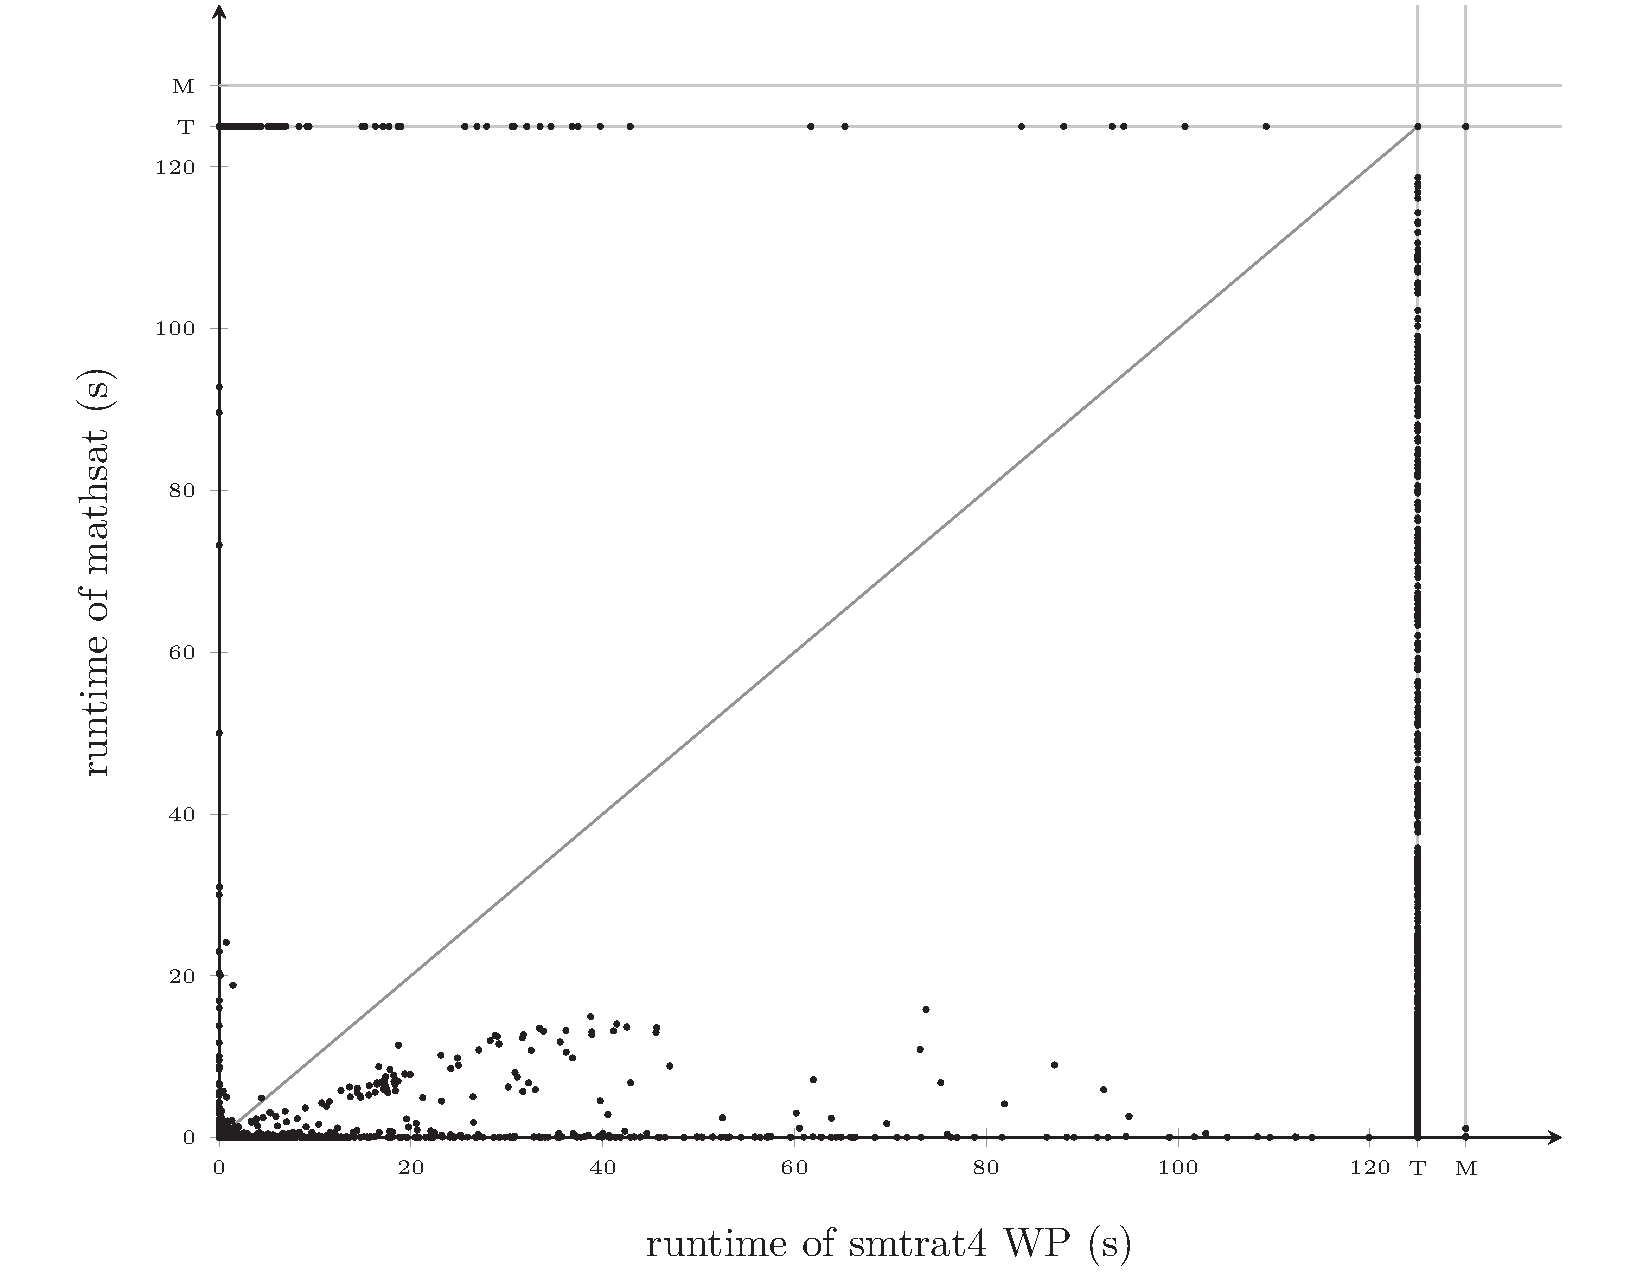
\includegraphics[width=1\linewidth]{./figures/scatter-smtrat_4_preprocessing-mathsat.pdf}
    % \scatterplot{smtrat4 WP}{mathsat}{scatter-smtrat_4_preprocessing-mathsat.data}
  \label{fig:Scatter_plot_for_smtrat4_WP_and_mathsat}
\end{figure}

\begin{figure}[!ht]
    \centering
    \caption{Scatter plot for smtrat4 WP and z3}
    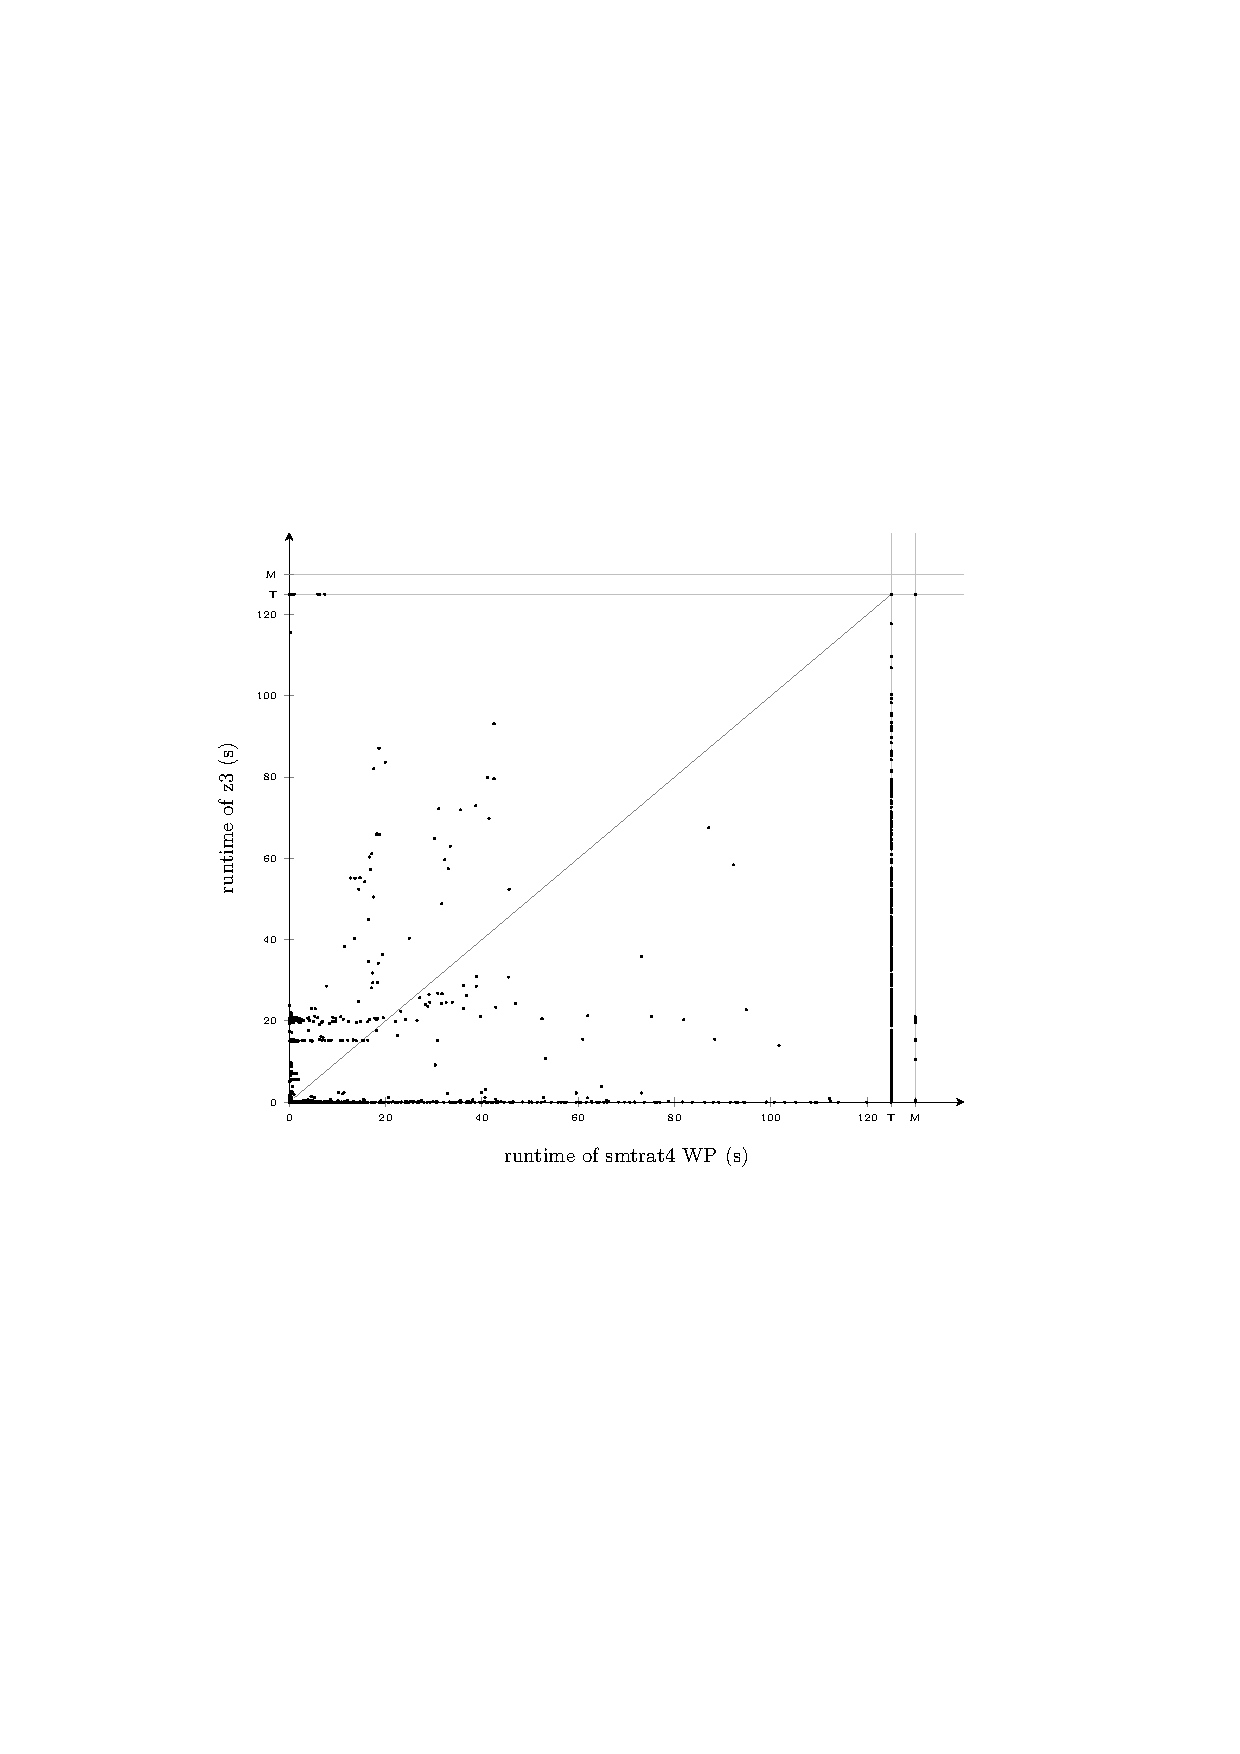
\includegraphics[width=1\linewidth]{./figures/scatter-smtrat_4_preprocessing-z3.pdf}
    % \scatterplot{smtrat4 WP}{z3}{scatter-smtrat_4_preprocessing-z3.data}
    \label{fig:Scatter_plot_for_smtrat4_WP_and_z3}
\end{figure}

\noindent We already know that we have defined three heuristic types and seven sequences of axiom types.
We have also seen that the a pair of heuristic type ALL and sequence $4$ can enhance the performance of a solver.
In other words, ICP has an influence on the enhancement of the performance.
That is why we think about to play around with the sequence by concentrating on ICP the highest.
So, for experimental purpose we create four additional SMT-RAT solvers (smtrat22, $\dots$, smtrat25) by switching on preprocessing with the following sequences of axiom types but with the same heuristic type ALL:

\begin{itemize}
    \item smtrat22 -> ICP, zero, tangent plane, congruence
    \item smtrat23 -> ICP, tangent plane, zero, congruence
    \item smtrat24 -> ICP, zero, ICP, tangent plane, ICP, congruence
    \item smtrat25 -> ICP, tangent plane, ICP, zero, ICP, congruence
\end{itemize}

\begin{table}[!ht]
\caption{Summary of smrat4, other additional smtrat solvers, mathsat and z3}
\begin{tabularx}{\textwidth}{lXrrXrrXrr}
	\toprule
	\textbf{Solver}
	&& \multicolumn{2}{c}{\textbf{SAT}}
	&& \multicolumn{2}{c}{\textbf{UNSAT}}
	&& \multicolumn{2}{c}{\textbf{overall}}
	\\
	\midrule
% 	smtrat4 (WoP)
% 	&& 1849 & 1.64~s
% 	&& 3914 & 1.67~s
% 	&& 5763 & 50.2~\%
% 	\\
% 	smtrat23 (WoP)
% 	&& 1948 & 0.59~s
% 	&& 4055 & 1.72~s
% 	&& 6003 & 52.2~\%
% 	\\
% 	smtrat22 (WoP)
% 	&& 1998 & 1.07~s
% 	&& 4035 & 1.63~s
% 	&& 6033 & 52.5~\%
% 	\\
% 	smtrat25 (WoP)
% 	&& 1956 & 1.10~s
% 	&& 4108 & 1.83~s
% 	&& 6064 & 52.8~\%
% 	\\
% 	smtrat24 (WoP)
% 	&& 2003 & 0.97~s
% 	&& 4100 & 1.57~s
% 	&& 6103 & 53.1~\%
% 	\\
	smtrat4 WP
	&& 2336 & 1.55~s
	&& 4348 & 2.41~s
	&& 6684 & 58.2~\%
	\\
	smtrat23 WP
	&& 2438 & 0.61~s
	&& 4449 & 2.31~s
	&& 6887 & 59.9~\%
	\\
	smtrat25 WP
	&& 2401 & 0.87~s
	&& 4490 & 2.50~s
	&& 6891 & 60.0~\%
	\\
	smtrat22 WP
	&& 2465 & 0.63~s
	&& 4443 & 2.39~s
	&& 6908 & 60.1~\%
	\\
	smtrat24 WP
	&& 2463 & 0.92~s
	&& 4463 & 2.40~s
	&& 6926 & 60.3~\%
	\\
	mathsat
    	&& 3560 & 1.20~s
     	&& 5286 & 1.80~s
     	&& 8846 & 76.9~\%
	\\
	z3
	&& 4985 & 0.36~s
	&& 5091 & 0.78~s
	&& 10076 & 87.7~\%
	\\
	\bottomrule
\end{tabularx}
\label{table:Summary_of_smrat4_and_other_additional_smtrat_solvers}
\end{table}

\noindent We exclude the axiom type monotonicity from the sequence for each of these solvers as monotonicity is the most costly to generate.
The results are reported in Table \ref{table:Summary_of_smrat4_and_other_additional_smtrat_solvers} which maintains the same structure as Tables \ref{table:results_our_solvers} and \ref{table:smtrat4_vs_mathsatAndZ3}.
It is highly visible that the total number of solved instances has increased the most for smtrat24 WP than smtrat4 WP and the increment is $3\%$.
As a result, the difference of overall performances between our solver and mathsat has decreased from $19\%$ to $17\%$.
Notice that smtrat24 follows almost the same pattern of the sequence $4$ except that ICP is inserted after each different axiom type in its sequence.
Figures \ref{fig:Scatter_plot_for_smtrat24_WP_and_mathsat} and \ref{fig:Scatter_plot_for_smtrat24_WP_and_z3} are the scatter plots for smtrat24 WP with mathsat and z3, respectively.
These two scatter plots have the same behaviour as like the scatter plots for smtrat4 WP with mathsat (Figure \ref{fig:Scatter_plot_for_smtrat4_WP_and_mathsat}) and z3 (Figure \ref{fig:Scatter_plot_for_smtrat4_WP_and_z3}), respectively.s\newline

\begin{figure}[]
    \centering
    \caption{Scatter plot for smtrat24 WP and mathsat}
    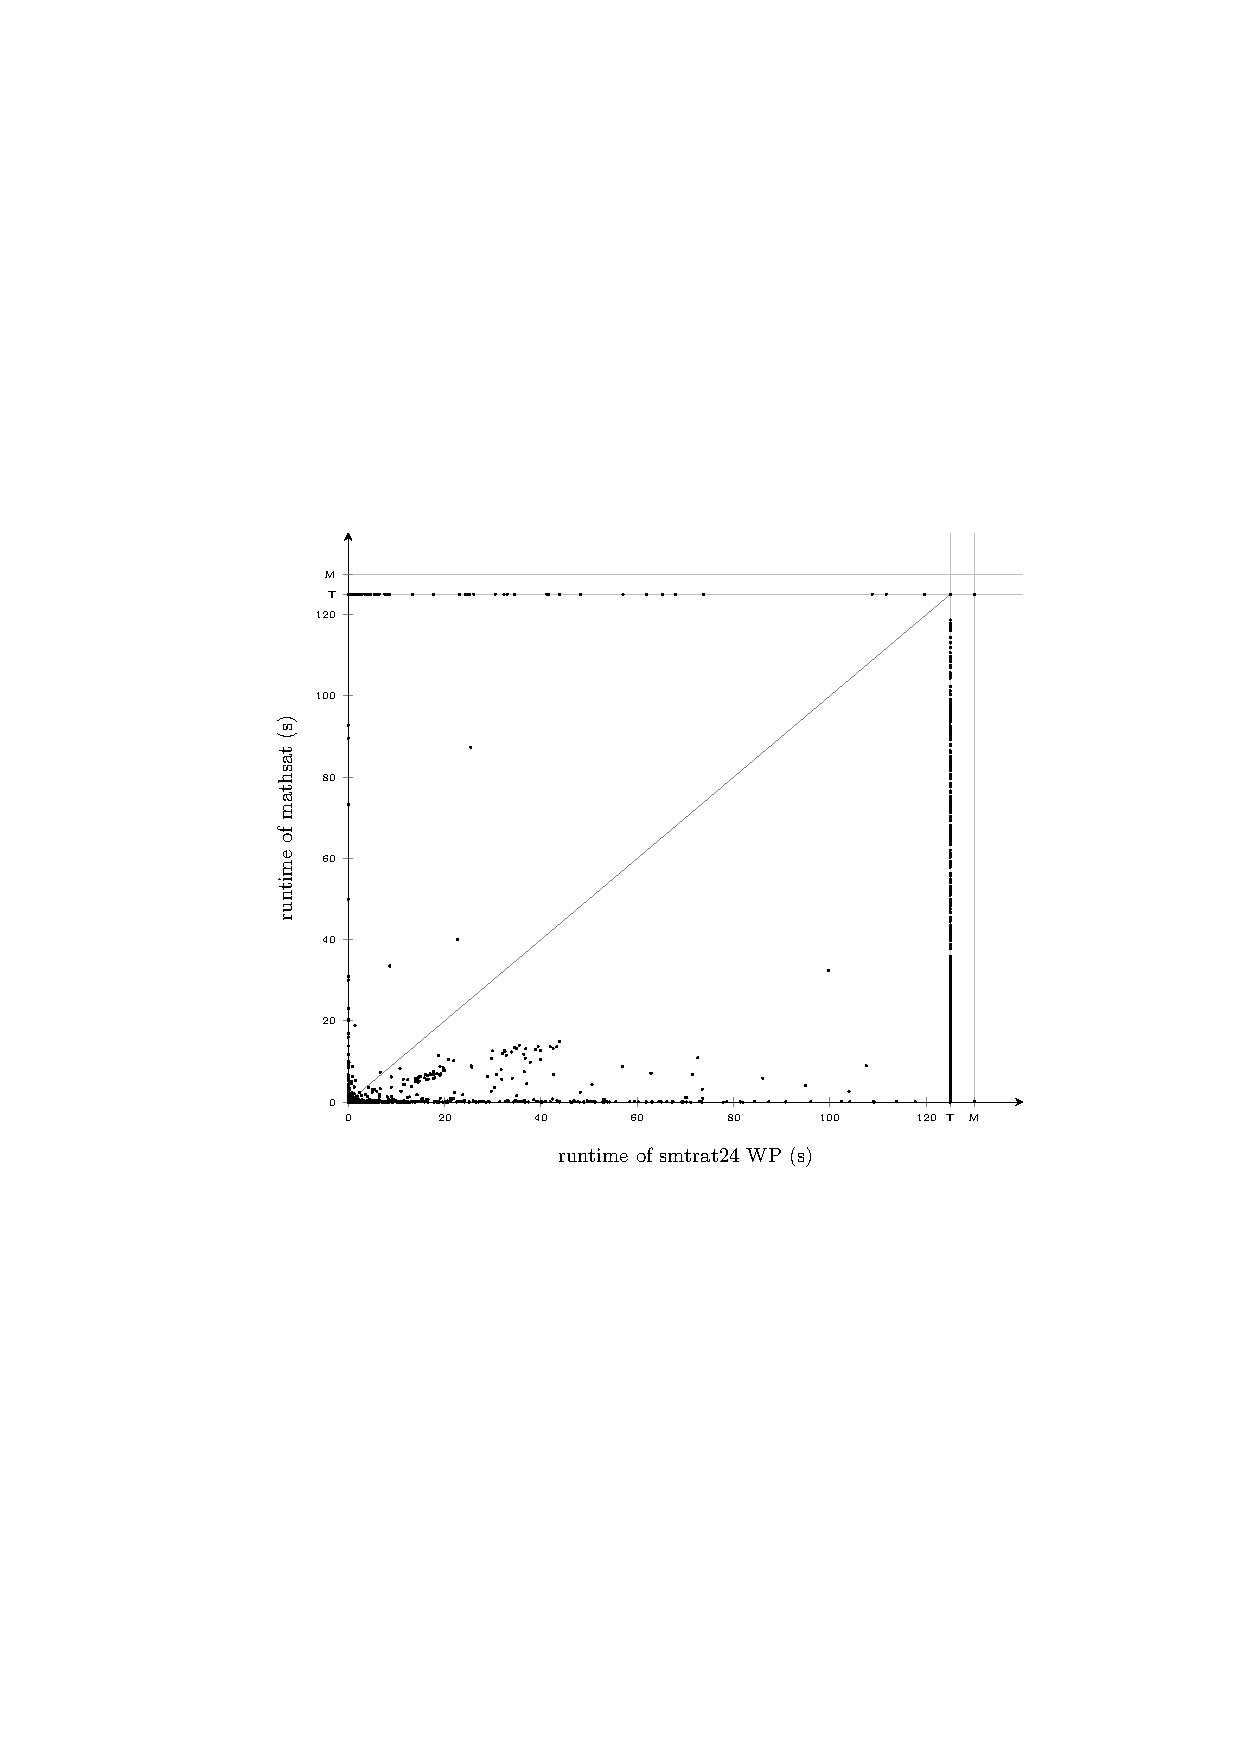
\includegraphics[width=1\linewidth]{./figures/scatter-smtrat_24_preprocessing-mathsat.pdf}
    % \scatterplot{smtrat4 WP}{mathsat}{scatter-smtrat_24_preprocessing-mathsat.data}
  \label{fig:Scatter_plot_for_smtrat24_WP_and_mathsat}
\end{figure}

\begin{figure}[]
    \centering
    \caption{Scatter plot for smtrat24 WP and z3}
    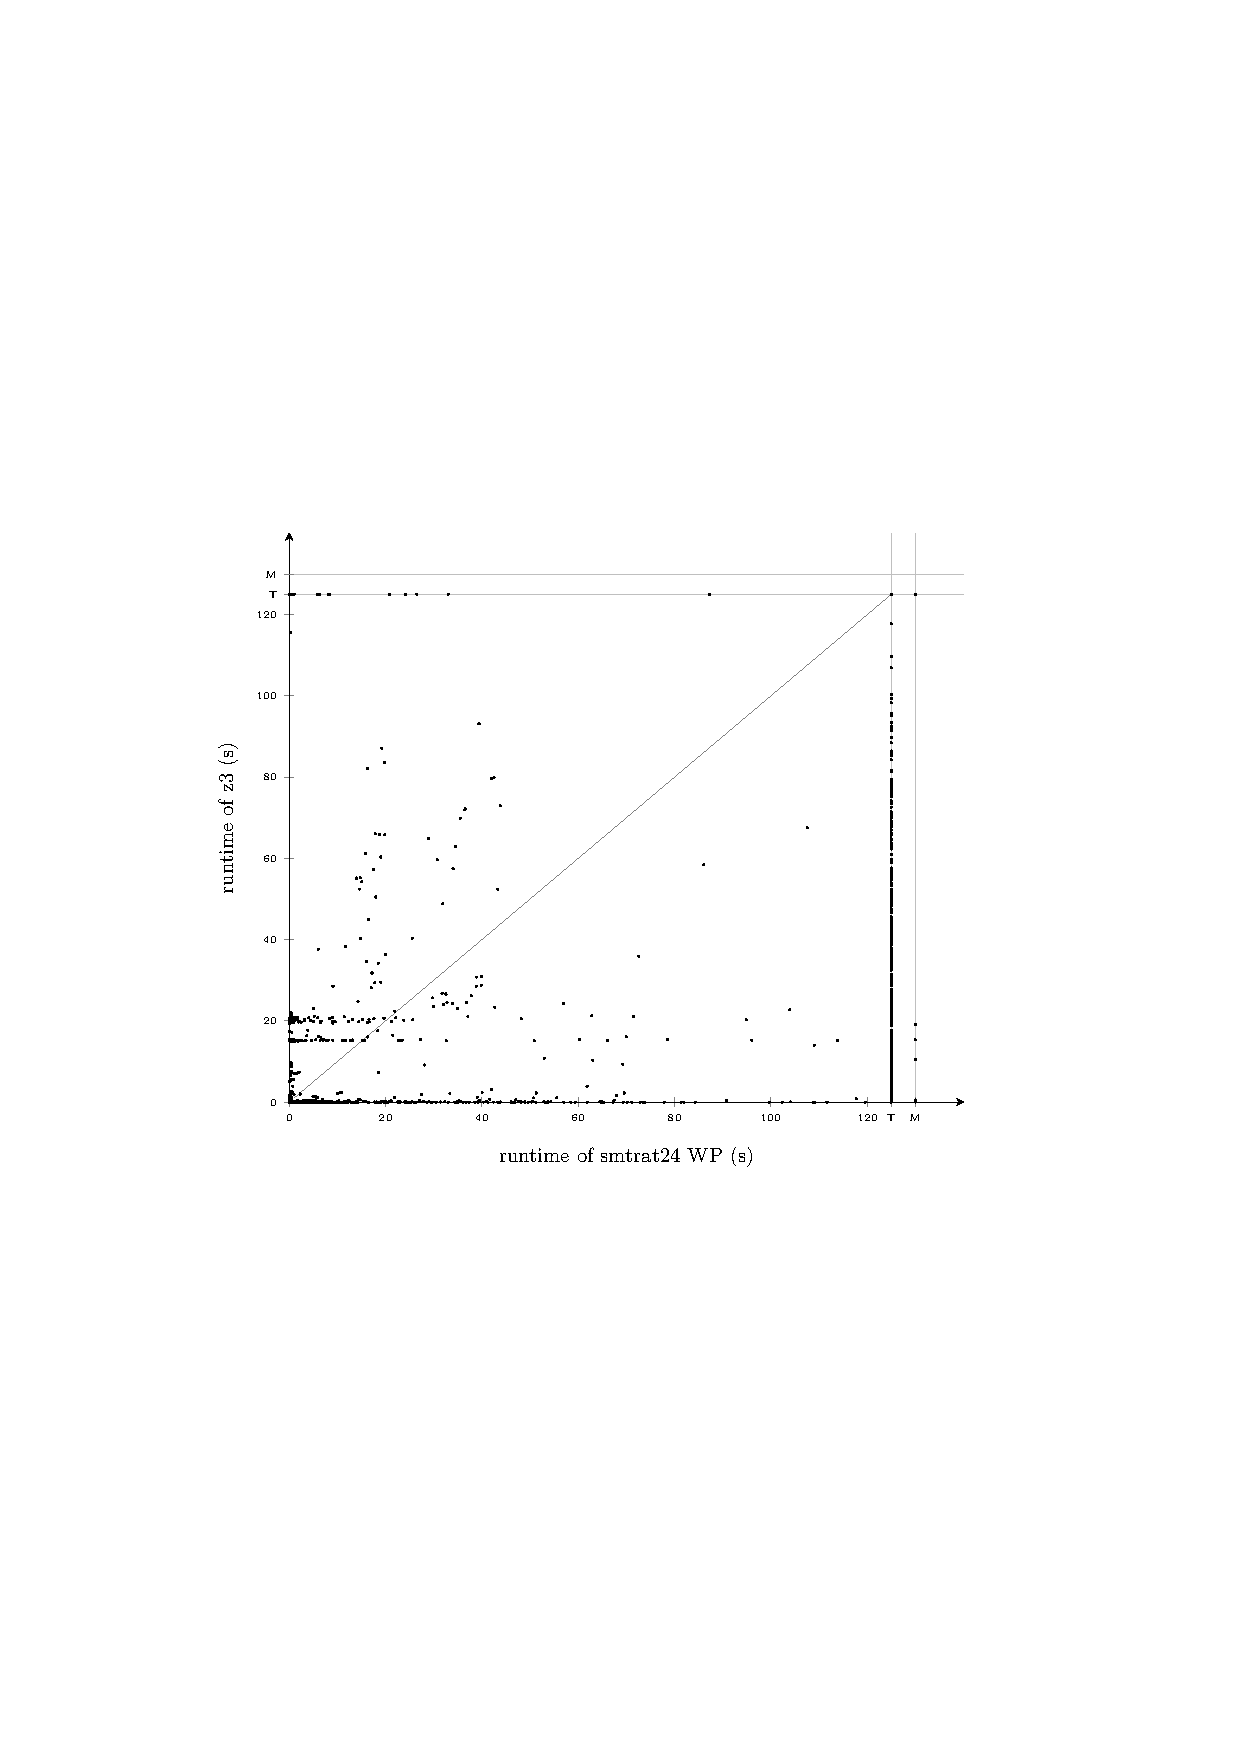
\includegraphics[width=1\linewidth]{./figures/scatter-smtrat_24_preprocessing-z3.pdf}
    % \scatterplot{smtrat4 WP}{z3}{scatter-smtrat_24_preprocessing-z3.data}
    \label{fig:Scatter_plot_for_smtrat24_WP_and_z3}
\end{figure}


